

\tikzset{every picture/.style={line width=0.75pt}} %set default line width to 0.75pt        

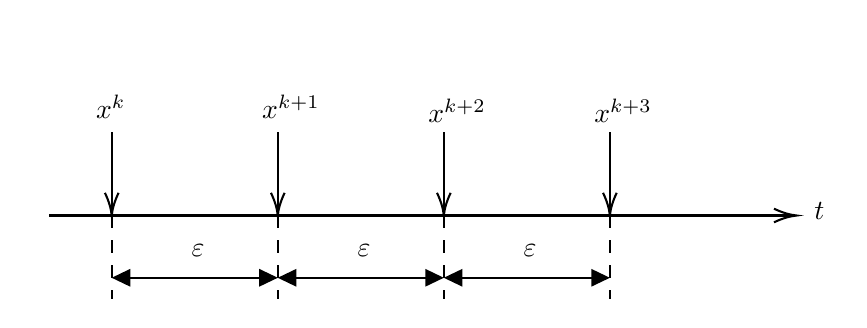
\begin{tikzpicture}[x=0.75pt,y=0.75pt,yscale=-1,xscale=1]
%uncomment if require: \path (0,300); %set diagram left start at 0, and has height of 300

%Straight Lines [id:da4879951122895062] 
\draw    (10,90) -- (368,90) ;
\draw [shift={(370,90)}, rotate = 180] [color={rgb, 255:red, 0; green, 0; blue, 0 }  ][line width=0.75]    (10.93,-3.29) .. controls (6.95,-1.4) and (3.31,-0.3) .. (0,0) .. controls (3.31,0.3) and (6.95,1.4) .. (10.93,3.29)   ;
%Straight Lines [id:da6973519196452055] 
\draw    (40,50) -- (40,88) ;
\draw [shift={(40,90)}, rotate = 270] [color={rgb, 255:red, 0; green, 0; blue, 0 }  ][line width=0.75]    (10.93,-3.29) .. controls (6.95,-1.4) and (3.31,-0.3) .. (0,0) .. controls (3.31,0.3) and (6.95,1.4) .. (10.93,3.29)   ;
%Straight Lines [id:da37258372717815214] 
\draw    (120,50) -- (120,88) ;
\draw [shift={(120,90)}, rotate = 270] [color={rgb, 255:red, 0; green, 0; blue, 0 }  ][line width=0.75]    (10.93,-3.29) .. controls (6.95,-1.4) and (3.31,-0.3) .. (0,0) .. controls (3.31,0.3) and (6.95,1.4) .. (10.93,3.29)   ;
%Straight Lines [id:da6922585100312479] 
\draw    (200,50) -- (200,88) ;
\draw [shift={(200,90)}, rotate = 270] [color={rgb, 255:red, 0; green, 0; blue, 0 }  ][line width=0.75]    (10.93,-3.29) .. controls (6.95,-1.4) and (3.31,-0.3) .. (0,0) .. controls (3.31,0.3) and (6.95,1.4) .. (10.93,3.29)   ;
%Straight Lines [id:da8649476764757188] 
\draw    (43,120) -- (117,120) ;
\draw [shift={(120,120)}, rotate = 180] [fill={rgb, 255:red, 0; green, 0; blue, 0 }  ][line width=0.08]  [draw opacity=0] (8.93,-4.29) -- (0,0) -- (8.93,4.29) -- cycle    ;
\draw [shift={(40,120)}, rotate = 0] [fill={rgb, 255:red, 0; green, 0; blue, 0 }  ][line width=0.08]  [draw opacity=0] (8.93,-4.29) -- (0,0) -- (8.93,4.29) -- cycle    ;
%Straight Lines [id:da07027249230414545] 
\draw    (123,120) -- (197,120) ;
\draw [shift={(200,120)}, rotate = 180] [fill={rgb, 255:red, 0; green, 0; blue, 0 }  ][line width=0.08]  [draw opacity=0] (8.93,-4.29) -- (0,0) -- (8.93,4.29) -- cycle    ;
\draw [shift={(120,120)}, rotate = 0] [fill={rgb, 255:red, 0; green, 0; blue, 0 }  ][line width=0.08]  [draw opacity=0] (8.93,-4.29) -- (0,0) -- (8.93,4.29) -- cycle    ;
%Straight Lines [id:da49306868755986777] 
\draw  [dash pattern={on 4.5pt off 4.5pt}]  (40,90) -- (40,130) ;
%Straight Lines [id:da4941954626905687] 
\draw  [dash pattern={on 4.5pt off 4.5pt}]  (120,90) -- (120,130) ;
%Straight Lines [id:da435515110639233] 
\draw  [dash pattern={on 4.5pt off 4.5pt}]  (200,90) -- (200,130) ;
%Straight Lines [id:da4247825385679421] 
\draw    (280,50) -- (280,88) ;
\draw [shift={(280,90)}, rotate = 270] [color={rgb, 255:red, 0; green, 0; blue, 0 }  ][line width=0.75]    (10.93,-3.29) .. controls (6.95,-1.4) and (3.31,-0.3) .. (0,0) .. controls (3.31,0.3) and (6.95,1.4) .. (10.93,3.29)   ;
%Straight Lines [id:da6033872749323609] 
\draw  [dash pattern={on 4.5pt off 4.5pt}]  (280,90) -- (280,130) ;
%Straight Lines [id:da04263965775882406] 
\draw    (203,120) -- (277,120) ;
\draw [shift={(280,120)}, rotate = 180] [fill={rgb, 255:red, 0; green, 0; blue, 0 }  ][line width=0.08]  [draw opacity=0] (8.93,-4.29) -- (0,0) -- (8.93,4.29) -- cycle    ;
\draw [shift={(200,120)}, rotate = 0] [fill={rgb, 255:red, 0; green, 0; blue, 0 }  ][line width=0.08]  [draw opacity=0] (8.93,-4.29) -- (0,0) -- (8.93,4.29) -- cycle    ;
%Straight Lines [id:da5149395390087544] 
\draw [color={rgb, 255:red, 255; green, 255; blue, 255 }  ,draw opacity=1 ]   (0,0) -- (390,0) ;

% Text Node
\draw (377,82.4) node [anchor=north west][inner sep=0.75pt]    {$t$};
% Text Node
\draw (31,30.4) node [anchor=north west][inner sep=0.75pt]    {$x^{k}$};
% Text Node
\draw (111,30.4) node [anchor=north west][inner sep=0.75pt]    {$x^{k+1}$};
% Text Node
\draw (191,32.4) node [anchor=north west][inner sep=0.75pt]    {$x^{k+2}$};
% Text Node
\draw (11,52.4) node [anchor=north west][inner sep=0.75pt]    {$\dotsc $};
% Text Node
\draw (311,52.4) node [anchor=north west][inner sep=0.75pt]    {$\dotsc $};
% Text Node
\draw (77,102.4) node [anchor=north west][inner sep=0.75pt]    {$\varepsilon $};
% Text Node
\draw (157,102.4) node [anchor=north west][inner sep=0.75pt]    {$\varepsilon $};
% Text Node
\draw (271,32.4) node [anchor=north west][inner sep=0.75pt]    {$x^{k+3}$};
% Text Node
\draw (237,102.4) node [anchor=north west][inner sep=0.75pt]    {$\varepsilon $};


\end{tikzpicture}
